\documentclass[10pt,a4paper,oneside]{article}
\usepackage[utf8]{inputenc}
\usepackage{amsmath}
\usepackage{amsfonts}
\usepackage{amssymb}
\usepackage{graphicx}
\usepackage{breqn}
\usepackage{tikz} % system block diagram
\usepackage{textcomp}
\usetikzlibrary{datavisualization}
\usetikzlibrary{shapes,arrows} % system block diagram
\usepackage{booktabs}
\usepackage[framed,numbered,autolinebreaks,useliterate]{mcode} % matlab code block
\author{Yangang Cao}
\date{February 25, 2019}
\newcommand{\degree}{^\circ}
\tikzset{
	delay/.style    = {draw, thick, rectangle, minimum height = 3em,
		minimum width = 3em},
	sum/.style      = {draw, circle, node distance = 2cm}, 
	prod/.style     = {draw, circle, node distance = 2cm},
	input/.style    = {coordinate}, % Input
	output/.style  = {coordinate} % Output
}
% Defining string as labels of certain blocks.
\newcommand{\product}{$\displaystyle \times$}
\newcommand{\delay}{\large$z^{-1}$}
\begin{document}

\title{Nonlinear Processing}
\maketitle 

The terms nonlinear processing or nonlinear processors are used for all signal processing algorithms or signal processing devices in the analog or digital domains which do not satisfy the condition of linearity. A system with input $x(n)$ and output $y(n)$ is called 	linear if the property
\[
x(n) = Ax_1(n) + Bx_2(n) \rightarrow y(n) = Ay_1(n) + By_2(n)
\]
is fullfilled. In all other cases it is called nonlinear. Nonlinear processing create intentional or untentional harmonic or inharmonic frenquency components which are not present in the input signal, this is what we called harmonic distorstion.\\

A measurement of the total harmonic distortion(THD) gives an indication of the nonliearnity of the system. Total harmonic distortion is defined by
\[
\mathrm{THD} = \sqrt{\frac{A_2^2 + A_3^2 + \cdots + A_N^2}{A_1^2 + A_2^2 + \cdots + A_N^2}},
\]
which is the square root of the radio of the sum of powers of all harmonic frenquency above the fundamental frequency to the power of all harmonics frequencies, including the fundmental frequency.\\

Dynamics processing is performed by amplifying devices where the gain is automatically controlled by the level of the input signal. We will discuss limiters, compressors, expanders and noise gates. \\

Dynamics processing is based on an amplitude/level detection scheme sometimes called an envelope follower, a static curve to derive a gain factor from the result of the envelope follower, a smoothing filter to prevent too abrupt gain changes and a multiplier to weight the input signal. Optionally, the input signal is delayed to compensate for any delay in the side chain. Normally, the gain factor is derived from the input signal, but the side chain path can also be connected to another signal for controlling the gain factor of the input signal.
\begin{center}
	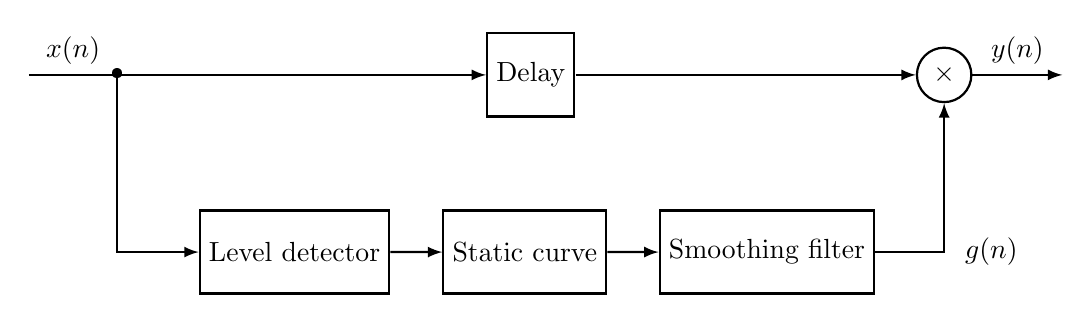
\begin{tikzpicture}[auto, thick, node distance=0.6cm, >=latex, scale = 0.75]
	\draw
	node at (7,0)[delay] (d1) {Delay} 
	node at (14,0)[prod] (p1) {\product}
	node at (3,-3)[delay](d2){Level detector}
	node at (6.9,-3)[delay](d3){Static  curve}
	node at (11,-3)[delay](d4){Smoothing filter}
	node at (14,-3)  (a)[] {} node [right of = a ]{$g(n)$};
	
	\draw[-](-1.5,0) -- node {$x(n)$} (0,0);
	\draw[->](p1) -- node {$y(n)$} (16,0);
	\draw[->](0,0) |- (d2);
	\draw[->](d2) -- (d3);
	\draw[->](d3) -- (d4);
	\draw[->](d4) -| (p1);
	\draw[->](0,0) -- (d1);
	\draw[->](d1) -- (p1);
	\draw node at (0,0) {\textbullet};
	\end{tikzpicture}
	\textbf {Figure} 
\end{center}
The level detector follows one of the two approaches :
\begin{itemize}
\item A full-wave rectifier in combination with an AR-averager with very short attack time may be used to track the peak value of the signal.
\item A square averaged with only a single time-constant provides the RMS value, measuring the signal's power.
\end{itemize}

\begin{center}
	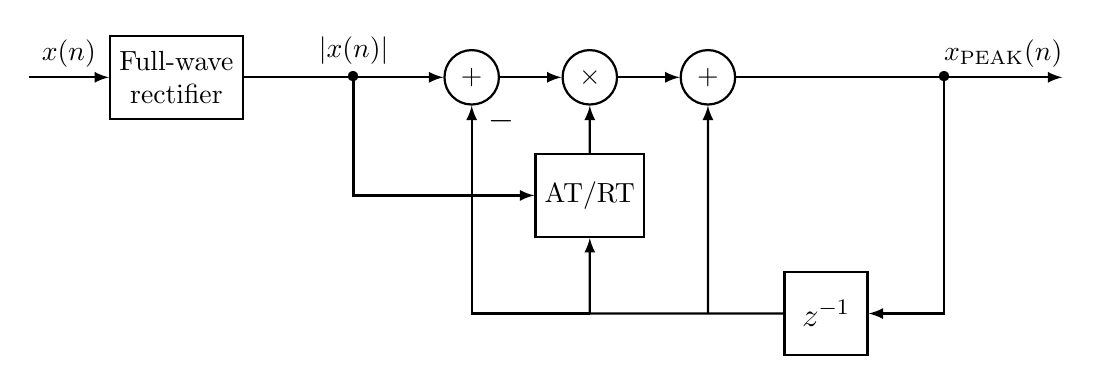
\begin{tikzpicture}[auto, thick, node distance=0.6cm, >=latex, scale = 0.75]
	\draw
	node at (-1,0) [delay,align=center] (d1) {Full-wave \\rectifier}
	node at (2,-0.35) [] (a) {} node [above of = a] {$\left|x(n)\right|$}
	node at (4,0) [sum] (s1) {+}
	node at (6,0) [prod] (p1) {\product}
	node at (8,0) [sum] (s2) {+}
	node at (6,-2) [delay] (d2){AT/RT}
	node at (10,-4) [delay] (d3) {\delay}
	node at (4.5,-0.75) {\large$-$};
	
	\draw[->](-3.5,0)--node {$x(n)$} (d1);
	\draw[->](d1)--(s1);
	\draw[->](s1)--(p1);
	\draw[->](p1)--(s2);
	\draw[->](2,0)|-(d2);
	\draw[->](6,-4)--(d2);
	\draw[->](6,-4)-|(s1);
	\draw[-](6,-4)--(d3);
	\draw[->](8,-4)--(s2);
	\draw[->](d2)--(p1);
	\draw[->](12,0)|-(d3);
	\draw[-](s2)--(12,0);
	\draw[->](12,0)--node {$x_{\mathrm{PEAK}}(n)$}(14,0);
	
	\draw node at (2,0) {\textbullet};
	\draw node at (12,0) {\textbullet};
	
	\end{tikzpicture}
	\textbf {Figure} Peak measurement for a dynamic range controller.
\end{center}
\begin{center}
	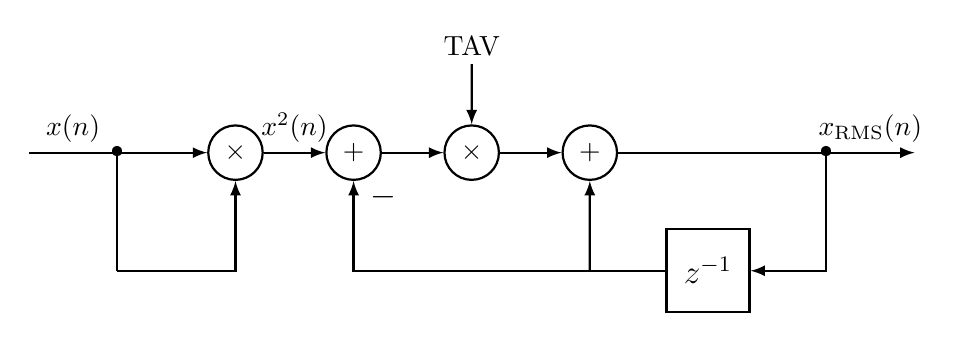
\begin{tikzpicture}[auto, thick, node distance=0.6cm, >=latex, scale = 0.75]
		\draw
		node at (2,0) [prod] (p1) {\product}
		node at (4,0)[sum] (s1) {+}
		node at (6,0) [prod] (p2) {\product}
		node at (8,0) [sum] (s2) {+}
		node at (10,-2) [delay] (d1) {\delay}
		node at (4.5,-0.75){\large$-$}
		node at (6,1.8) {TAV};
		
		\draw[-](-1.5,0)--node {$x(n)$} (0,0);
		\draw[->](0,0)--(p1);
		\draw[-](0,0)--(0,-2);
		\draw[->](0,-2)-|(p1);
		\draw[->](p1)--node{$x^2(n)$}(s1);
		\draw[->](s1)--(p2);
		\draw[->](6,1.5)--(p2);
		\draw[->](d1)-|(s1);
		\draw[->](p2)--(s2);
		\draw[-](s2)--(12,0);
		\draw[->](8,-2)--(s2);
		\draw[->](12,0)--node {$x_{\mathrm{RMS}}(n)$} (13.5,0);
		\draw[->](12,0)|-(d1);
		
		\draw node at (0,0) {\textbullet};
		\draw node at (12,0) {\textbullet};
		
	\end{tikzpicture}
	\textbf {Figure} RMS measurement for a dynamic range controller.
\end{center}
The static curve decides which function(limiter, compressor, expander,\dots) the dynamic range controller emploies. It is best described on a dB scale, so we introduce $X$, $G$ and $Y$ for the levels of the respective signals in dB. The multiplication at the dynamic range controller’s output then becomes $Y = X + G$.\\

The dynamic behavior of a dynamic range controller is influenced by the level measurement approach (with attack AT and release time RT for peak measurement and averaging time TAV for RMS measurement) and further adjusted with a smoothing filter.
\end{document}
